\section{Rank Aggregation}
\label{sec:methods:rank}

Now that we have seen how to adaptively aggregate scalar scores, it is time to see how
to do \emph{adaptive rank aggregation}. Rank aggregation means combining sorted lists of items.
In this scenario, each modeling method takes the current user as input, and produces a
list of items ranked in order of rating
(see Section \ref{sec:theory:rank}).

Aggregating lists is desirable in a number of situations:
Often we wish to produce lists of recommended items, not just estimate the rating of a single combination.
Consider the task of personalizing a list of search results
(see Section \ref{sec:search}). The important part is not the score
given to each result, but rather the order in which they appear.
The underlying technology is still the same: a number of recommenders are used to predict the ratings
of items to users. However, to do rank aggregtion, another layer is added, that requests lists from each method,
not only singular items.

Because it is such an important use case, we shall use personalized search to present our approach to adaptive rank aggregation.
In addition to the standard recommenders, we have an information retrieval method,
as introduced in Section \ref{sec:ir}.
The IR method takes in a user-initiated query (a collection of words or a sentence), and returns a number of 
search results, in an ordered list.
In traditional personalized search, a recommender system can then be used to estimate a rating for each of the returned items,
and re-sort, or re-score, the results list (e.g. \citet[p3]{Xu2008}).

The key insight is that both the IR method and the recommender systems form \emph{input signals}
(see Section \ref{subsec:signals}).
An input signal is some measure of how each item should be ranked in the final results list.
The relevance scores returned from our IR ranking functions are signals,
and the predicted ratings from each recommender systems are signals.
Adaptive aggregation then entails estimating \emph{how accurate ach of these signals are likely to be for the current user and item}.
This is almost the same task as in adaptive prediction aggregation, only in a list-oriented fashion.

The important difference is this: The IR methods constrict the range of items worked on by the recommender systems.
As the IR methods identify items that may be relevant to the users query, these are the items we wish the recommender systems to work on.
This goes back to the previously mentioned difference between \emph{search} and \emph{recommendations}:

\begin{itemize*}
  \item Recommenders find relevant items the user does not already know exists.
  \item Search engines find relevant items the user knows or hopes exists.
\end{itemize*}

The difference lies in the knowledge of existence.
As personalized search is still a search task, the IR methods should determine the set of items that might be relevant.
Their relevance scores for these items becomes the first input signals.
The recommender systems works on this set of items, rescoring each as needed.
We still have the adaptive layer that estimates how well each signal will perform for the current user and item.
This is especially important considering that we may have multiple IR methods that define multiple sets of relevant items.
The final result is an adaptive combination of the rating and accuracy preictions for each signal,
as seen in Figure \ref{fig:adaptiverank}.
Let us now see how the modeling and prediction phases are performed in adaptive rank aggregation.

\begin{figure}[t]
  \center
  \def\layersep{3cm}
  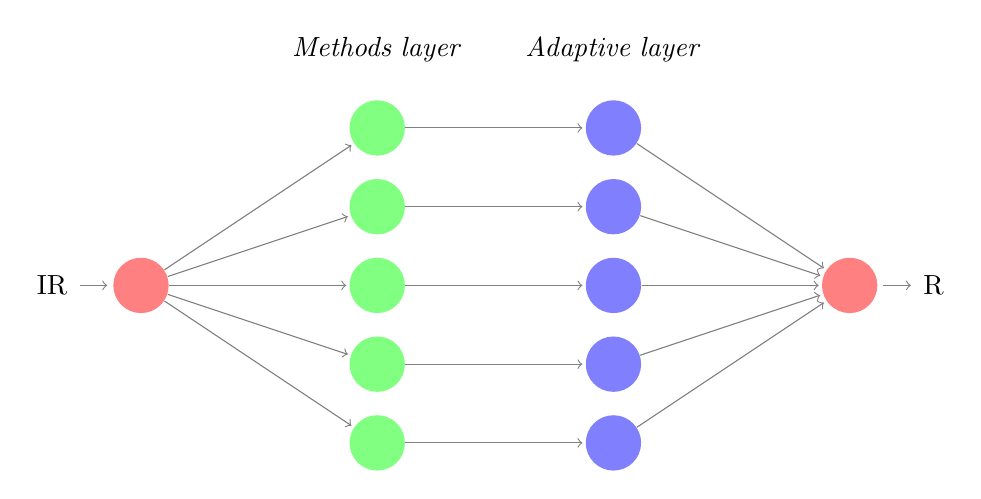
\begin{tikzpicture}[shorten >=1pt,->,draw=black!50, node distance=\layersep]

    \tikzstyle{every pin edge}=[<-,shorten <=2pt]
    \tikzstyle{neuron}=[circle,fill=black!25,minimum size=20pt,inner sep=0pt]
    \tikzstyle{input neuron}=[neuron, fill=green!50];
    \tikzstyle{output neuron}=[neuron, fill=red!50];
    \tikzstyle{hidden neuron}=[neuron, fill=blue!50];
    \tikzstyle{annot} = [text width=10em, text centered]
    
    \node[output neuron, pin=left:IR] (IR) at (0,-3) {};
    
    \node[input neuron] (M-1) at (\layersep, -1) {};
    \node[input neuron] (M-2) at (\layersep, -2) {};
    \node[input neuron] (M-3) at (\layersep, -3) {};
    \node[input neuron] (M-4) at (\layersep, -4) {};
    \node[input neuron] (M-5) at (\layersep, -5) {};
    
    \node[hidden neuron] (E-1) at (\layersep*2, -1) {};
    \node[hidden neuron] (E-2) at (\layersep*2, -2) {};
    \node[hidden neuron] (E-3) at (\layersep*2, -3) {};
    \node[hidden neuron] (E-4) at (\layersep*2, -4) {};
    \node[hidden neuron] (E-5) at (\layersep*2, -5) {};
    
    \node[output neuron,pin={[pin edge={->}]right:R}, right of=E-3] (O) {};
    
    \foreach \source in {1,...,5}
         \path (M-\source) edge (E-\source);
     
    \foreach \source in {1,...,5}
         \path (IR) edge (M-\source);
 
    \foreach \source in {1,...,5}
         \path (E-\source) edge (O);
    
    \node[annot, above of=M-1, node distance=1cm] (hl) {\emph{Methods layer}};
    \node[annot, right of=hl] {\emph{Adaptive layer}};

  \end{tikzpicture}

  \vspace{1em}
  \caption[Stacked Rank Aggregation]{
    Stacked Rank Aggregation: 
    An IR method returns a results list of possibly related items, each with a ranking score.
    The methods layer estimates ratings for each item in the results list.
    The adaptive layer predicts how accurate ach of these ratings are likely to be.
    Finally, the ranking scores, ratings and accuracy estimations are combined
    into one result list, R.
  }
  \label{fig:adaptiverank}
\end{figure}


\subsection{Modeling Phase}

We shall only deal with settings where we have a single IR method.
While multiple IR methods and corresponding error models would be an interesting
setting, we are most interested in using the IR method for constraining the Item-space considered by the recommender systems.
As we shall see, this does not introduce many changes to our previously developed algorithms.

The modeling phase for the recommender system stays the same, with one important change.
As we are dealing with a search engine, we might not have an explicit ratings matrix to rely on.
Most feedback we can gather from user initiated searches are from query logs.
These logs show the current user, query, and the item that is finally selected after the query is performed.
Query log mining is a common approach in personalized search
(e.g. \cite{Liu2002, Sugiyama2004, Shen2005, Speretta2000}).
By mining this log, we can create an implicit ratings matrix.
Each populated cell represents a selected item.

The values in this implict ratings matrix can take many forms.
If we only care about selected items, binary ratings may suffice:
selected items are then represented by a $1$ in the ratings matrix.
These ratings can be further improved by considering different metrics, including:

\begin{itemize*}
  \item Time spent before selecting the item.
  \item How far the user was willing to scroll before clicking the item.
  \item Whether or not the user resubmitted the same query shortly after.
\end{itemize*}

Based on these, and similar, metrics, we can achieve quite accurate implicit ratings.
Naturally, ratings can also be gathered from other sources.
If we have more data on each user, or know of secondary systems such as social networks
or other systems where ratings are present, these can be used to augment the implicit ratings matrix
(e.g. \cite{Carmel2009}).
There are also search systems where we already have explicit ratings:
Consider, for instance, the use case of searching for movies on a movie rating site,
or searching for people in a social network.
In these cases, we have explicit ratings that can be used to train the recommender models.

A thorough explanation of turning query logs into ratings matrices
is beyond the scope of this thesis. Extensive research already
looks at how implicit user model information may be gleaned
from simple query logs. Examples include \cite{Joachims2007},
\cite{Lee2005}, \cite{Agichtein2006}, \cite{Mobasher} and
\cite{Speretta2000}.

When we have the implicit or explicit ratings matrix, the modeling phase
consists of two parts: training the IR models and the recommender models.
The recommender models are trained as before, given in Listing \ref{code:training}.
The one or more IR methods are not trained with a ratings matrix,
but with the items and their respective data.
Of course, the actual IR modeling method depends on the IR system itself,
which is not our concern in this chapter.


\subsection{Prediction Phase}

\begin{algorithm}[t]
  \begin{algorithmic}[1]
  \REQUIRE user: The current user
  \REQUIRE items: The set of all items and their meta-data
  \REQUIRE query: The user initiated query
  \REQUIRE ir\_model: A trained IR model
  \REQUIRE rating\_models: The set of trained modeling methods 
  \REQUIRE error\_models: The set of trained error models
  \ENSURE
    \STATE $ratings \gets \emptyset$
    \STATE $errors  \gets \emptyset$
    \STATE $results \gets \mathrm{Search}(ir\_model, items, query)$
    
    \FORALL{$item \in results$}
      \FORALL{$m \in rating\_models$}
        \STATE $ratings_{m,item} \gets \mathrm{Predict}(rating\_models_m, user, item)$
        \STATE $errors_{m,item}  \gets \mathrm{Predict}(error\_models_m, user, item)$
      \ENDFOR 
    \ENDFOR
    \STATE $errors \gets \mathrm{Normalize}(errors)$

    \FORALL{$item, ir\_score \in results$}
      \STATE $prediction \gets w_{IR} \times ir\_score$
      \FORALL{$m \in rating\_models$}
        \STATE $weight_{item} \gets 1 - error_{m,item}$
        \STATE $prediction \gets prediction + weight_m \times ratings_{m,item}$
      \ENDFOR
      \STATE $item_{prediction} \gets prediction$
    \ENDFOR
    
    \STATE $results \gets \mathrm{SortByPredictions}(results)$
  \RETURN $results$

  \end{algorithmic}
  \caption[Adaptive Rank Aggregation]{Adaptive Rank Aggregation}
  \label{code:rank:prediction}
\end{algorithm}

The prediction phase is where adaptive rank aggregation differs most from adaptive prediction aggregation.
Listing \ref{code:rank:prediction} gives the basic algorithm.
As input, instead of one item, we have the entire set of items, and a query.
We run the query and items through the IR model to get the constrained set of items ($results$).
Each of the recommender methods is then run for each of the items in the results list.
As before, the first for-loop can easily be peformed in parallel.
Each call to $\mathrm{Predict}$ is independent of the other operations,
allowing us to perform it as a $\mathrm{map}$ operation.

As before, the error estimations are normalized before converting them to weights.
Since we are dealing with two dimensions of errors, for each item and each method,
the errors are normalized across items.
In other words, for each item, the errors from the recommenders fall in the range $[0,1]$ and sum to $1$.

After each item in the results list has an IR score, a set of predictions, and a corresponding set of 
error predictions, the adaptive aggregated prediction is computed. 
Because we do not care of the final score we set the initial predictions to be the IR scores.
The recommender systems simply add or substract from this initial score.
This means that the resulting predictions will not be in the same range as the known ratings,
but since we are only interested in the order of the items, not the actual rating, this poses no problem.

An important coefficient is the $w_{IR}$ (IR weight),
which determines how much the IR method should decide of the final ranking.
This is first and formost adjusted to ensure that the IR scores
are on a similar scale as the predicted ratings.
At the same time, this weight determines how 
much the IR score influences the final placement of an item in the results list.
In the next chapter, we shall see how the choice this parameter 
influences the ranked results lists.

After computing the predictions for each item in the results list, 
we sort the list by the item predictions, and return the list.
The resulting list is adaptively sorted based on the current user and the specific items in the list,
achieving in adaptive rank aggregation.

Clearly, as in prediction aggregation, the strength of our resulting system is in large part dependent on the accuracy of our ratings.
This means that deciding and understanding how implicit ratings are created, or 
finding auxiliary sources to provide explicit ratings, is a critical step.
As we have said before, algorithms are only as strong as the data they can leverage.
In other words, methods for personalized search will work best in settings where we have explicit ratings,
or can gather explicit ratings from secondary sources, for example from external social networks or publishing platforms.


